\documentclass[a4paper,12pt]{article} % Changer la taille de police c'est ici

\usepackage{framed} % Marges
\usepackage[utf8]{inputenc} %francais
\usepackage[T1]{fontenc} %francais
\usepackage[french]{babel}  %francais
\usepackage{lmodern} % Pour changer le pack de police
\usepackage{makeidx} % Index
\usepackage{graphicx} % Figures
\usepackage{wrapfig} % Figures
\usepackage{amsmath} % Maths
\usepackage{amssymb} % symboles ?
\usepackage{bclogo} % ?????
\usepackage{stmaryrd}
\usepackage[top=2cm, bottom=2cm, left=2cm, right=2cm]{geometry} %Marges

\title{Rapport Tache 2 (partie 2)}
\author{Interpolaspline}
\date{Avril 2020}

\begin{document}

\maketitle

\section{Implémentation}

\subsection{Méthode de calcul numérique}

Le programme a pour principal but de trouver la valeur des dérivées en chaque noeuds pour pouvoir appliquer le procédé d'interpolation d'Hermite.

Pour se faire, on utlise le résultat donné plus haut, donnant la relation entre les données, les noeuds de lissage et les dérivées cherchées.

Ainsi, la majorité des fonctions du programme est constituée par de la définition de matrices en fonction de paramètres.

\subsection{tests}

Les tests ont été réalisés sur des cas précis et sur un jeu de cas aléatoires.

\begin{itemize}
\item[•] Cas d'une distribution uniforme : On retrouve le même résultat que lors de tests sur le programme de la tache 1. (Figure \ref{unif})
\item[•] Cas d'une distribution de Chebichev (Figure \ref{cheb})
\item[•] Cas aléatoires : On remarque comme attendu que si la distribution est trop chaotique, alors l'interpolante ne sera plus forcément optimisée. Cela dépend beaucoup des données. (Figures \ref{normal},\ref{euh} et \ref{aled})
\end{itemize}

\begin{figure}
\begin{center}
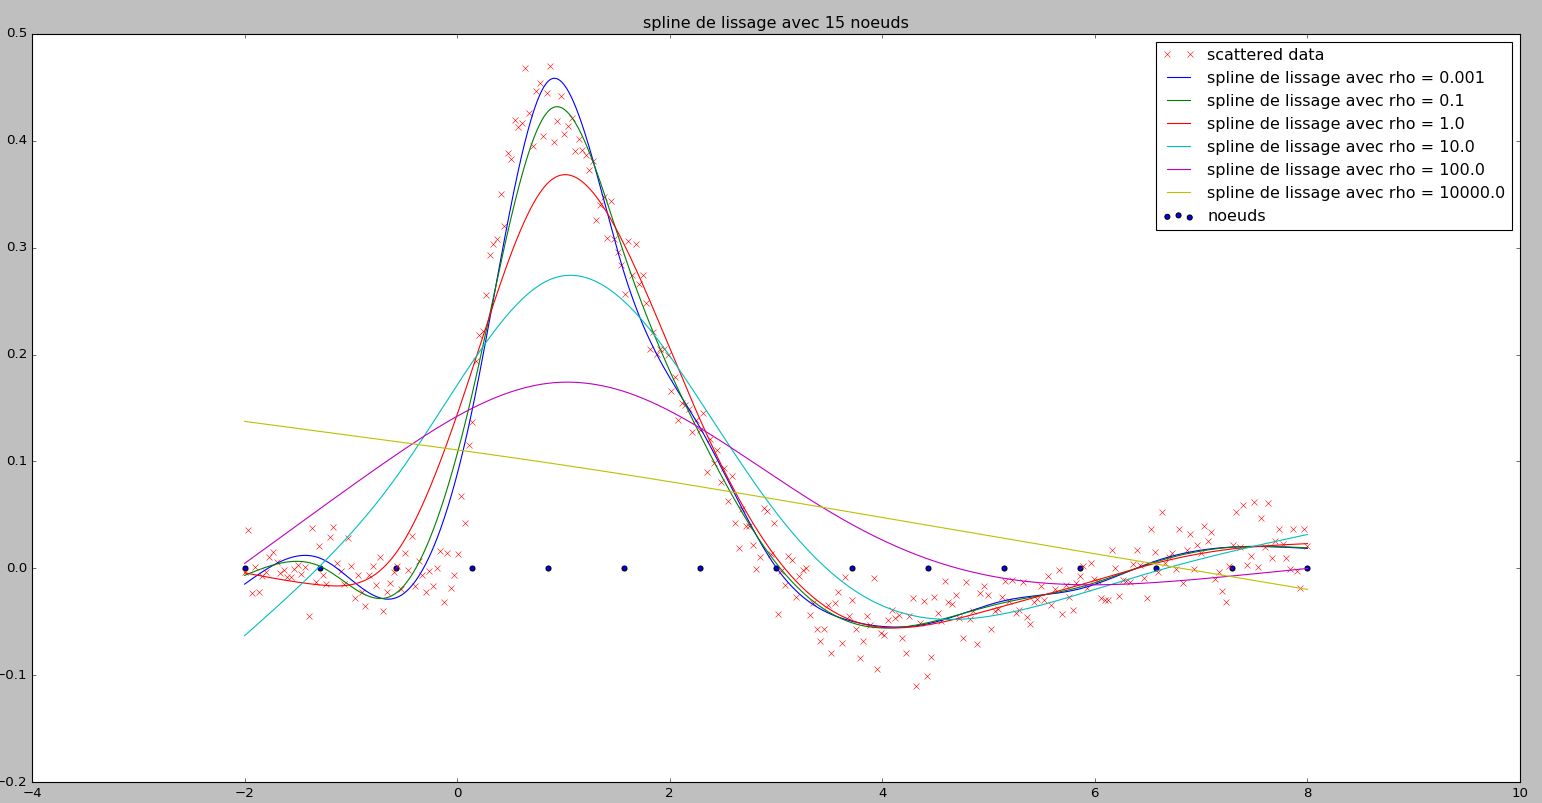
\includegraphics[width=8cm]{unif.png} 
\end{center}
\caption{Exemple sur une répartition uniforme}
\label{unif}
\end{figure}

\begin{figure}
\begin{center}
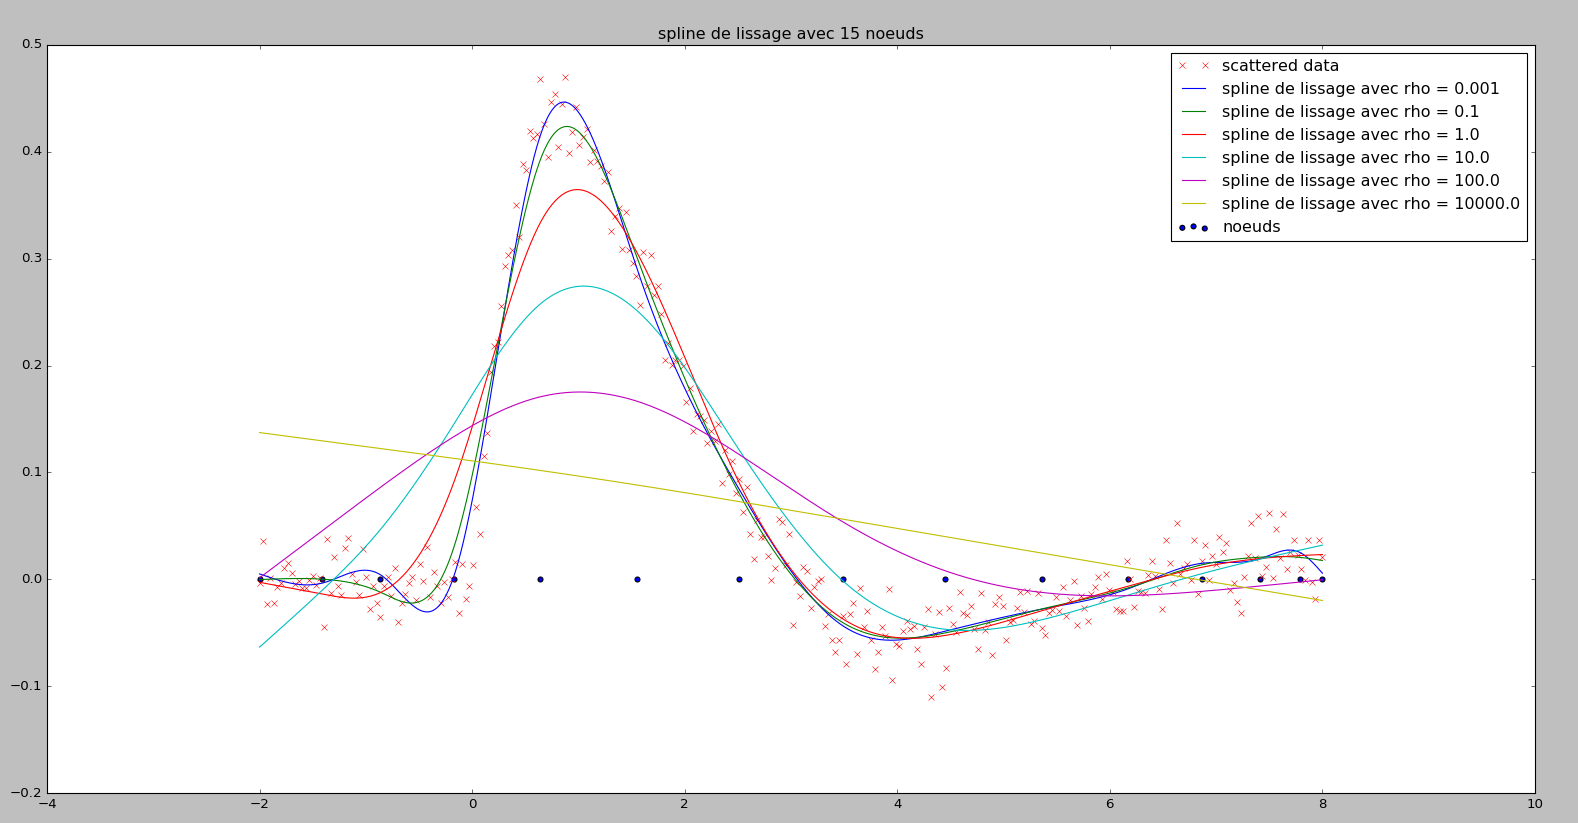
\includegraphics[width=8cm]{Cheb.png} 
\end{center}
\caption{Exemple sur une répartition de Chebichev}
\label{cheb}
\end{figure}

\begin{figure}
\begin{center}
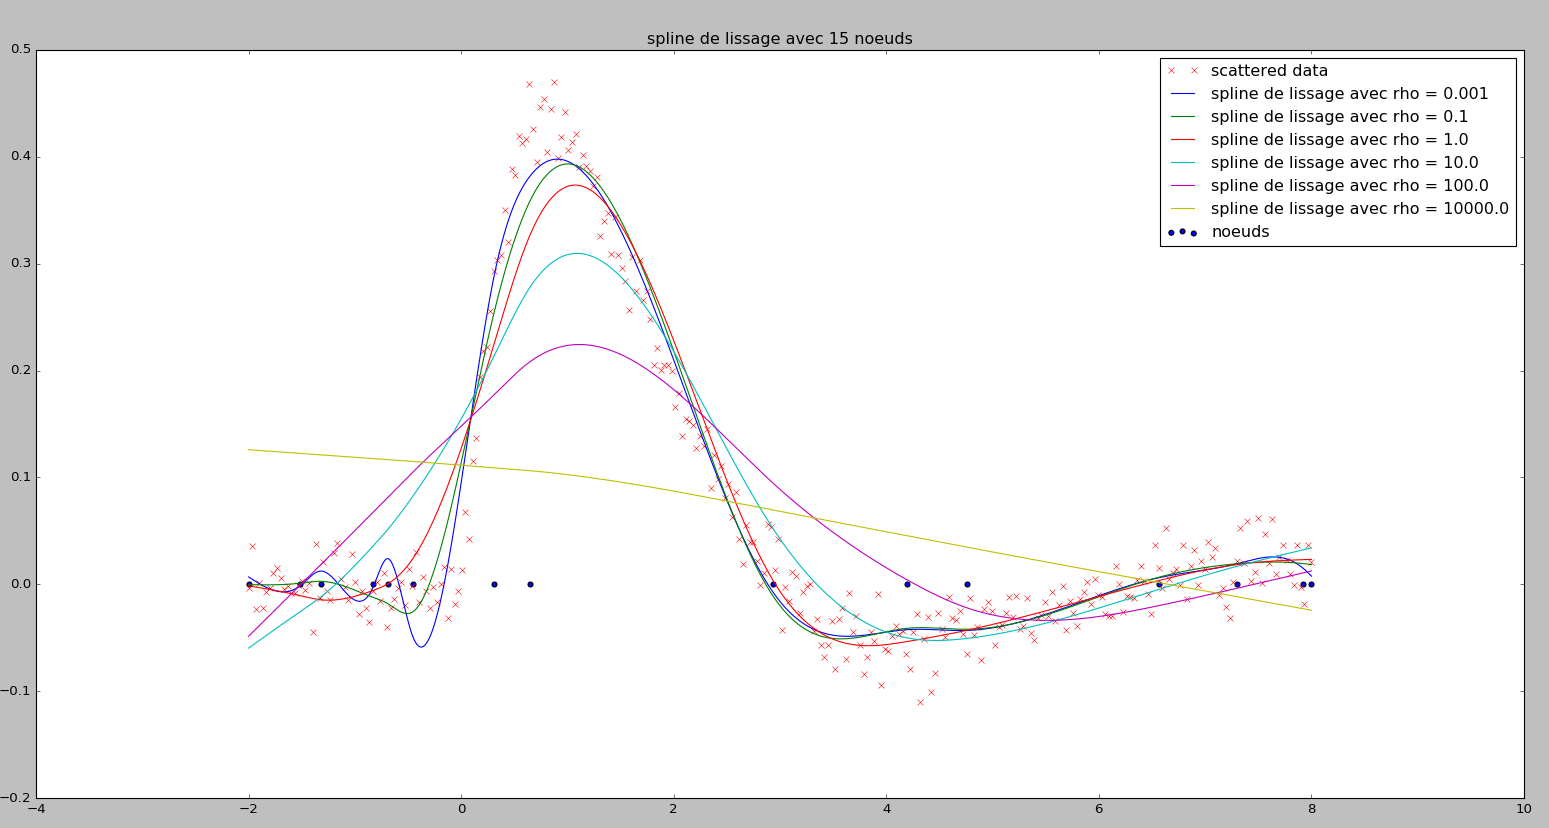
\includegraphics[width=8cm]{normal.png} 
\end{center}
\caption{Exemple sur une répartition alétatoire (1)}
\label{normal}
\end{figure}


\begin{figure}
\begin{center}
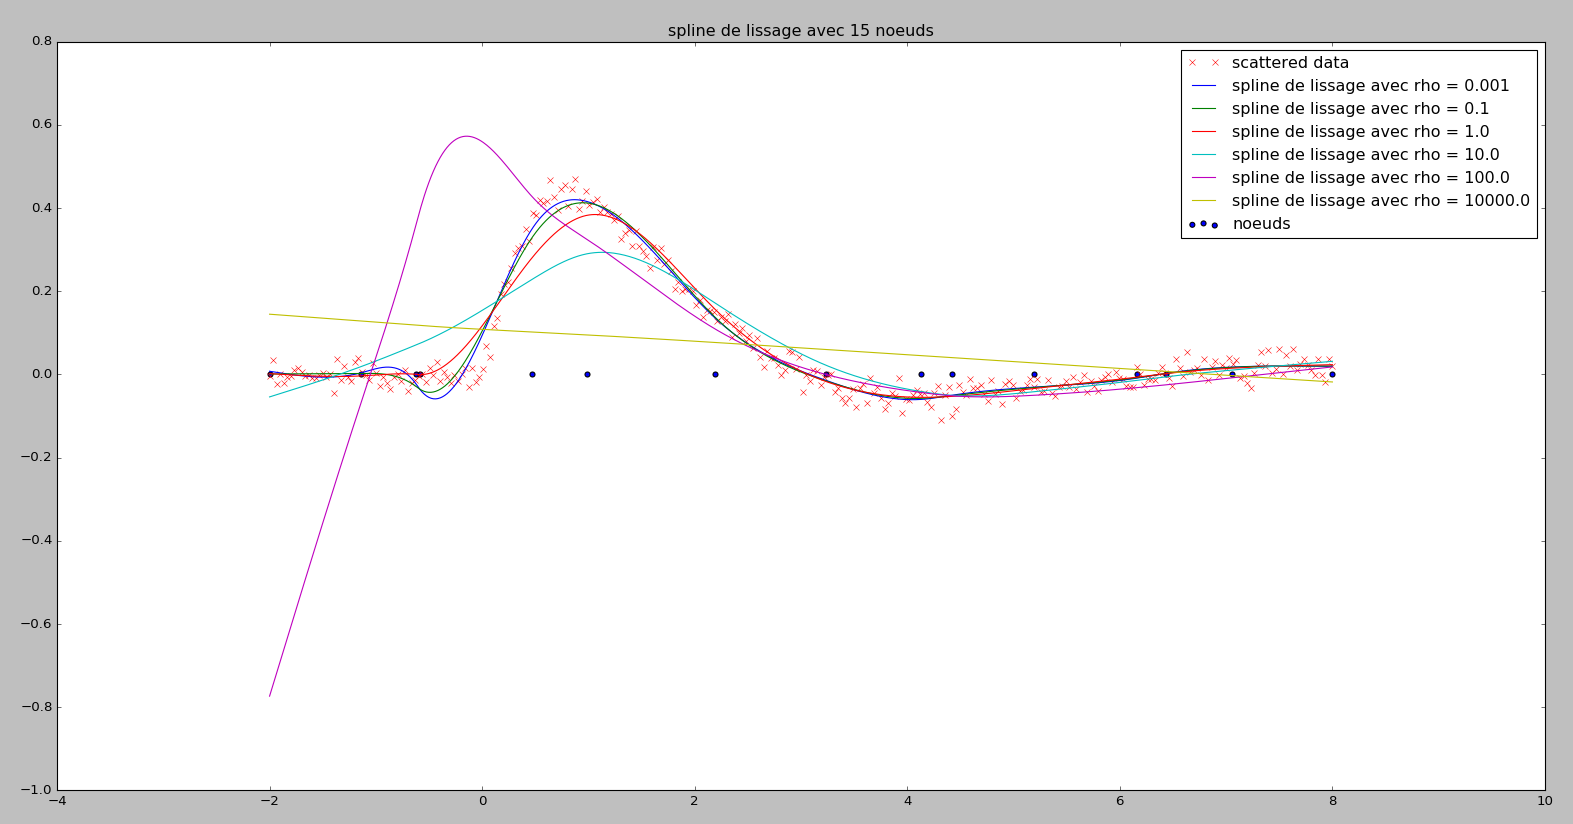
\includegraphics[width=8cm]{euh.png} 
\end{center}
\caption{Exemple sur une répartition alétatoire (2)}
\label{euh}
\end{figure}

\begin{figure}
\begin{center}
\includegraphics[width=8cm]{aled.png} 
\end{center}
\caption{Exemple sur une  répartition alétatoire (3)}
\label{aled}
\end{figure}

\end{document}
